\chapter{Estado del arte}

En este capítulo estudiaremos y analizaremos los diferentes enfoques para nuestra principal tarea, \textbf{la segmentación de tumores cerebrales}. Abordando desde el inicio del estudio del problema pasando por la explosión de métodos basados en Aprendizaje profundo con la constitución de \textbf{BraTS} hasta nuestros días. Se pondrá especial énfasis a las soluciones actuales comparándolas desde sus diferencias en metodología y perspectiva.

Otras tareas contenidas en el diagnóstico completo de tumores cerebrales como la clasificación de tumores cerebrales (glioblastomas y meningiomas) o la predicción de su evolución, que se recogen en este trabajo, van intrínsecamente unidas al buen desempeño de la tarea de segmentación. 

Por un lado, la clasificación entre los dos tipos de tumores no es tan relevante a la hora de diseñar un sistema de ayuda a la toma de decisión ya que clínicamente sí existe una característica diferencial entre ambos, su \textbf{localización}. Los meningiomas siempre aparecen entre el cráneo y el cerebro no internamente en el cerebro como los glioblastomas. Esto hace que un médico pueda distinguirlos sin requerir una gran asistencia de una máquina para la mayoría de los casos. Adicionalmente, la clasificación de por sí ayuda a la toma de decisiones en el tratamiento pero no es el elemento crítico para la supervivencia del paciente que depende de la eliminación del tumor donde su segmentación toma un papel crucial.

Por otro lado, la tarea de la predicción de la evolución del tumor se representa como la predicción de la segmentación en un estado futuro del tumor es decir depende fuertemente de la segmentación actual del tumor. 

Es por ello que grandes esfuerzos se han realizado en entorno a la segmentación, ya que otras tareas que conforman su diagnóstico se verían arrastradas.

Diferentes dificultades han sido las que a pesar de años de desarrollo aún encontrar un algoritmo para la segmentación de tumores cerebrales sea algo mejorable. 

\begin{enumerate}
	\item \textbf{Incertidumbre en la localización} : Como vimos no existe una zona concreta en general para la aparición de los tumores cerebrales. A excepción, de los meningiomas localizados en zonas superficiales del cerebro y aún siendo una región muy amplia, incluso ya desarrollado un tumor pueden aparecer otros localizados en regiones muy distintas de la original. 
	\item \textbf{Incertidumbre en la morfología} : A diferencia de otras patologías, cada tumor cerebral presenta un tamaño y forma completamente distintas y donde en principio no se puede apreciar un patrón distintivo. Esto hace que sea muy complicado y generalmente aporte malos resultados, la construcción de sistemas basados reglas u otras aproximaciones que no incluyen una componente de aprendizaje.
	
	\item \textbf{Bajo contraste} : Una buena resolución y contraste son características muy importantes para entender la información de una imagen. Las imágenes IRM producidas en una resonancia debido a proyecciones de imagen y procesos de tomografía usualmente ofrecen una baja resolución y contraste haciendo más difícil la definición de bordes entre diferentes tejidos de la imagen. Una segmentación precisa es difícil de conseguir.
	
	\item \textbf{Sesgo en las etiquetas}. Existen indicios para pensar que las etiquetas proporcionadas pueden presentar ruido. El proceso de segmentado por parte del personal médico 
	depende de su experiencia profesional lo cual puede llevar a cometer errores. Por ejemplo, se han presentado eventualmente discrepancias entre distintos anotadores: algunos tienden a conectar todas las pequeñas regiones de un tejido mientras que otros las segmentan de forma más precisa y separada. 
	
	\item \textbf{Desbalanceo en el tejido} : Dentro de la segmentación entre los diferentes tipos de tejidos, usualmente existe un tejido NCR que es usualmente más pequeño que los otros dos. 
	Esto podría afectar en el proceso de aprendizaje hacia una pobre generalización de este tipo de tejido. 
	
	\item \textbf{Desbalanceo entre pacientes} : En el conjunto de datos tenemos muchos pacientes de norteamerica y de ascendencia blanca, pero pocos de otros origenes como el africano. Además, de tener un sesgo claro de edad ya que existen pocos casos en niños. Esta falta de datos puede impedir que exista una buena generalización para estos casos más aislados.
	
\end{enumerate}



\section{Revisión histórica}

	A continuación, se presenta una revisión histórica sobre la segmentación de tumores cerebrales hasta 2021 apoyada en \cite{liu2023deep}. Se presenta una línea del tiempo con los principales trabajos de estudio.
	
	\begin{figure}[!h]
		\centering
		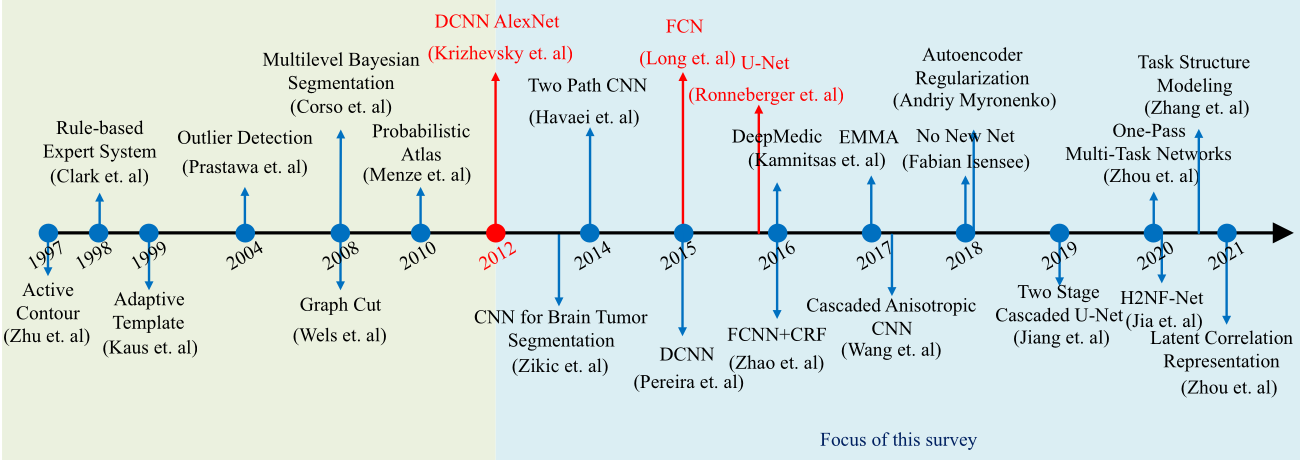
\includegraphics[width=1.0\linewidth]{imagenes/evolution_stateofart.png}
		\caption{Evolución histórica del estado del arte hasta 2021.}
	\end{figure}
	
	En la década de 1990 investigadores como Zhu et al. fueron pioneros al utilizar una red Hopfield con un modelo de contornos activos para extraer los bordes del tumor. Sin embargo, incluso el entrenamiento de una pequeña red como esta era algo computacionalmente costoso por las limitaciones de la época.  Desde 1990 hasta 2012, los métodos que iban surgiendo para la segmentación de tumores cerebrales estaban basados en métodos clásicos de aprendizaje con características extraídas a mano, sistemas expertos que se apoyaban en los histogramas de la imagen, plantillas para la segmentación y modelos gráficos. 
	
	A pesar de ser un gran paso inicial, tenían grandes deficiencias. Por ejemplo, la mayoría de ellos sólo se centraba en la segmentación de todo el tumor lo cual lleva a un modelo poco útil. Por otro lado, en los modelos basados en características extraídas se hacía muy tedioso poder usarlos eficazmente ya que este paso de extracción dependía de conocimiento previo experto que en ningún momento se pudo llegar a representar en un modelo. En último lugar, los mismos problemas que compartimos hoy en día sobre el desbalanceo y la incertidumbre del problema eran mucho más agresivos. 
	
	
	
	





\section{Enfoques actuales}
	\subsection{Basados en convolución}
	\subsection{Basados en Transformers}

